\chapter{Analyse causale}
\epigraph{Economists and agronomists are locked in debate about likely
future yields. Since the method of the economists is to predict
future outcomes from past performance, economists expect
success to continue. And since for the scientists future success
depends on discoveries they will have to make and do not now
know how to make, the scientists are doubtful. At its core, this is
a disagreement about the pace of technical change.}{Robert
Socolow}
\cleardoublepage

	\section{Introduction à la régression en composantes principales}
	Les méthodes de régression multivariée comme la RCP\footnote{Régression en composantes principales} jouissent d'une large popularité dans divers domaines d'études, y compris les sciences naturelles. La raison principale de ce succès étant qu'elle ont été conçues dans l'optique de faire face à des situations où on dispose de plusieurs variables exogènes, généralement hautement corrélées, et relativement peu d'échantillons. Une situation qui est justement notre problématique. Ainsi une forme de réduction de dimensions dans l'espace des exogènes peut grandement simplifier le problème de régression.L'analyse en composantes principales est une technique de réduction de dimensions où une combinaison linéaire de \textit{p} variables indépendantes/orthogonales des paramètres intrants $X_1,X_2,...X_p$ sont créées de façon à ce que la première combinaison linéaire $Z_{1}$ (composante principale) capture autant de la variance totale des données d'origine. La $2^{de}$ $Z_{2}$ capture autant que possible du reste de la variance sous la réserve que celle-ci soit orthogonale(i.e. non corrélée) à la première. En général toutes les variables intrantes sont standardisées de façon à posséder une moyenne nulle et une variance unitaire que l'on notera $X_{j}^{*}$. Ainsi la variance totale des \textit{p} intrants standardisés est donnée par :
	\begin{equation*}
	\sum_{j=1}^{p} V(X_{j}^{*}) = p = \sum_{j=1}^{p}V(Z_{j})
	\end{equation*}
	avec $\forall i \in [1,p]$:
	\begin{equation*}
	Z_i = \sum_{j=1}^{p} a_{ij} X_{j}^{*} 
	\end{equation*}
	et $\forall i \neq j$
	\begin{equation*}
		Cov(Z_i,Z_j) = Corr(Z_i,Z_j) = 0
	\end{equation*}
	Les composantes principales sont déterminées par l'analyse spectrale (i.e la recherche des valeurs propres et vecteurs propres) de la matrice des corrélations des variables intrantes. La variance de la $j^{eme}$ composante principale $Z_{j}$ est $\lambda_{j}$ la $j^{eme}$ valeur propre la plus grande. Les coefficients $a_{ij}$ de la combinaison linéaire sont les vecteurs propres correspondant.\par
	Idéalement les \textit{k} premières composantes principales comprendront une part consistante de la variance totale des données. Nous pouvons par la suite utiliser ces \textit{k} principales composantes $Z_1,Z_2,...X_k$ comme variables exogènes dans le modèle de régression linéaire multiple:
		\begin{equation*}
		Y=\beta_0 + \sum_{\j=1}^{k} \beta_jZ_j + \epsilon 
		\end{equation*}
	Dans ce qui suit nous mettons en œuvre une RCP sur nos données élaguées obtenus après le traitement du chapitre précédent. Le script en langage \textbf{R}, avec lequel la RCP est automatisée, est disponible dans le dossier \textit{Source} de notre dépôt PFE \textbf{GitHub}\cite{this}.
	\section{Mise en œuvre: corrélations croisées des variables exogènes}
	Nous commençons d'abord par charger les données quantitatives des pays. Il s'agit de l'élagage des données externes présentées à la section \ref{exoList}. Ces données représentent, de la totalité des 39 variables initiales, les 12 variables retenues en sortie de la procédure introduite par les forets aléatoires en section \ref{faout} avant de créer deux matrices:\begin{itemize}
	\item DF.actifs = Cette matrice accueillera les 12 variables retenues dans la figure \ref{fig:laggedvars}.
	\item DF.illus = Cette matrice-vecteur accueillera notre variable de sortie qui est la \textbf{Consommation de kilogrammes de fertilisants phosphatés par hectare de terre arable} 
	\end{itemize}
	Commençons d'abord à chercher les variables relativement colinéaires. Nous donnons dans la figure \ref{fig:scatter} les diagrammes de dispersions deux-à-deux croisés entre les 12 variables de notre modélisation. Nous joignons à ceux-ci des courbes splines facilitant la détection de structure ainsi qu'en gras les valeurs des coefficients de corrélations les plus importants.
			\begin{figure}[h]
				    		\centering
				    		\fbox{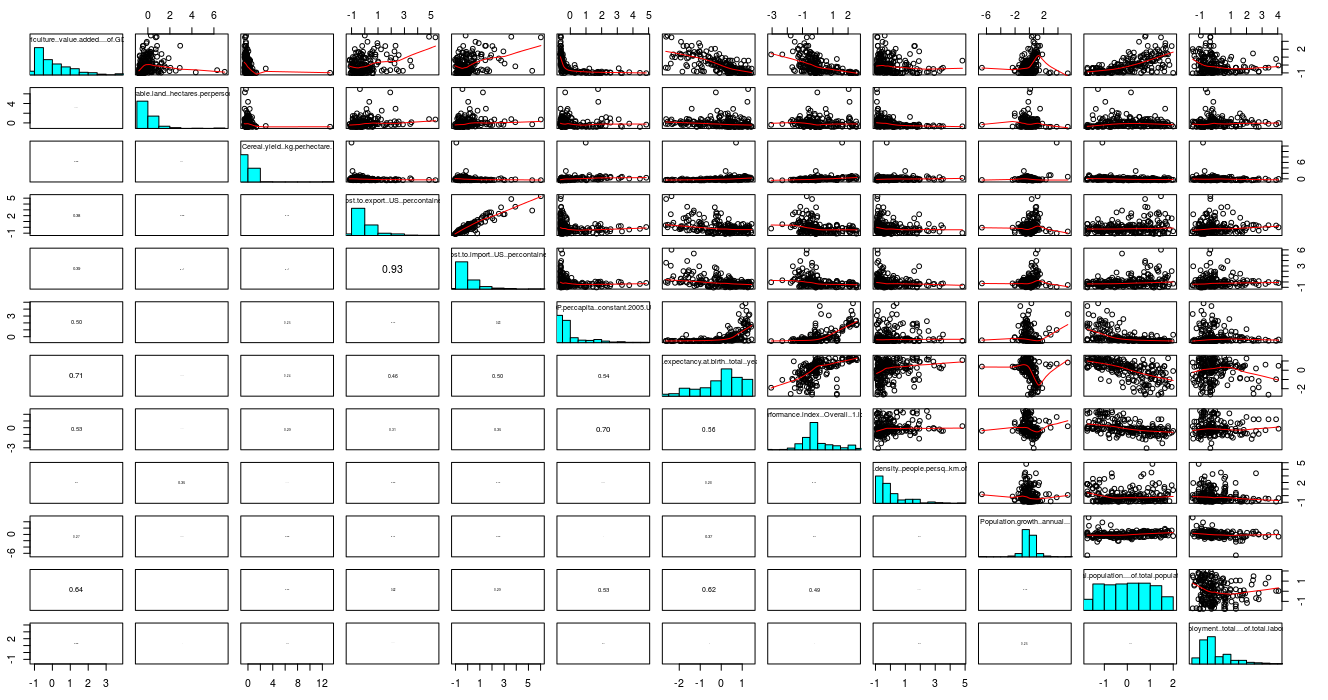
\includegraphics[width=\linewidth]{ch4-images/scatter}}
				    		\caption{Diagrammes des dispersions croisées, courbes splines et corrélations des variables exogènes}
				    		\label{fig:scatter}
			\end{figure}
	Plusieurs couples de valeurs présentent des corrélations sensiblement élevées en valeurs absolues:
	\begin{itemize}
	\item \{Coût d'import conteneur Vs Coût d'export conteneur\}
	\item \{\%(Agriculture) du PIB Vs Espérance de vie\}
	\item \{PIB par habitant Vs Indice de performance logistique\}
	\item \{\%(Agriculture) du PIB Vs \%(Population rurale) de la population totale\}
	\item \{Indice de performance logistique Vs Espérance de vie\}
	\item Certaines de ces variables entre elles par transition des couple ci-dessus.
	\end{itemize}
	Une autre façon d'examiner la structure des corrélations est la création de carte coloriée dressant les corrélations deux à deux entre les variables numériques. Ceci sont \textit{clusturisés} et ordonnés aux seins de groupes de variables corrélées. Sur la figure \ref{fig:heatmap} nous pouvons distinguer 4 à 5 groupes de variables exogènes corrélées. Ainsi une ACP devrait produire 4 à 5 composante principales intégrant la majorité de l'information contenue dans les données.
				\begin{figure}[H]
					    		\centering
					    		\fbox{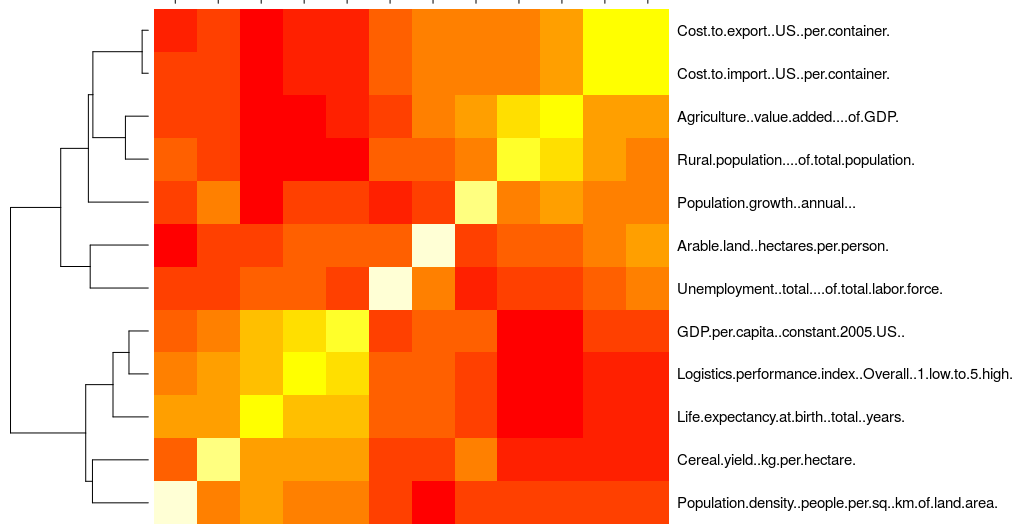
\includegraphics[width=\linewidth]{ch4-images/heatmap}}
					    		\caption{Carte coloriée des regroupement des variables corrélées}
					    		\label{fig:heatmap}
				\end{figure}
				Les groupes crées par le dendogramme ci-dessous donne un avant-goût des choses à venir. Il nous tente de deviner 3 familles de variables:\begin{itemize}
				\item \textbf{Des indicateurs de pressions démographiques:} Les variables \textit{Densité de population}, \textit{PIB par habitant} et \textit{Espérance de vie} communiquent sur la concentration, le pouvoir d'achat et la qualité de vie (et donc de nourriture) des gens dans un pays en question. Puisque le pouvoir d'achat ainsi que l’approvisionnement continu en matières premières est possible (\textit{Indice de la performance logistique)}, des pays réalisant de hauts scores dans les variables de cette famille, devraient en toute intuition, mener à une culture intensive des terres à dispositions-\textit{Rendement des céréales en kg par hectare}-. Ces \textit{5 variables} sont rassemblées par l'arbre inférieur de niveau 1 sur le dendrogramme de la figure \ref{fig:heatmap}
				\item \textbf{Des indicateurs de la structure industrielle:} La tendance d'un pays à importer de la marchandise dépend du coût des imports relativement à leur production chez soi. Plus la part de \textit{L'agriculture dans le PIB} augmente, moins le pays est industrialisé. De pair avec la \textit{Fraction des populations rurales des habitants},ceci informerait potentiellement sur la prépondérance de l'agriculture comme secteur clé ou secondaires au sein du pays. Ces \textit{3 variables} sont rassemblées par l'arbre supérieur de niveau 3 sur le dendrogramme de la figure \ref{fig:heatmap}
				\item \textbf{Des indicateurs de pressions écologiques:} Les \textit{surface arables par personne} est un rapport essentiel dans notre analyse. Il est évident que pour un pays disposant de peu de terres pour subvenir aux besoins alimentaires d'une grande population, une utilisation intensive d'engrais est à prévoir. L'arbre intermédiaire de niveau 2 du dendrogramme de la figure \ref{fig:heatmap} qui fait intervenir \textit{le taux de chômage} nous incite à nous poser la question de la capacité du consommateur à payer les frais d'une utilisation massive d'engrais pour sa nourriture.
				\end{itemize}
	Ces hypothèses ne sont pas forcément significatives, mais nous aurons dépoussiéré des pistes de réflexions pour élucider éventuellement les contributions de chaque variable au sein des CP en section \ref{fig:ZZ} que nous calculerons dans le paragraphe suivant : 
	\section{Mise en œuvre: calcul des composantes principales des données élaguées}
	Nous commençons par effectuer une décomposition spectrale de la matrice de corrélation. La figure \ref{fig:valpropres} ci-dessous liste les valeurs propres résultant de cette décomposition. Alors que la figure \ref{fig:scree} résume leur Scree-plot.
				\begin{figure}[H]
					    		\centering
					    		\fbox{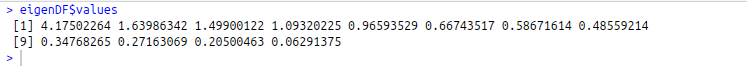
\includegraphics[width=\linewidth]{ch4-images/valeurs_propres}}
					    		\caption{Valeurs propres de la décomposition spectrale de la matrice de corrélation}
					    		\label{fig:valpropres}
				\end{figure}
					\begin{figure}[H]
						    		\centering
						    		\fbox{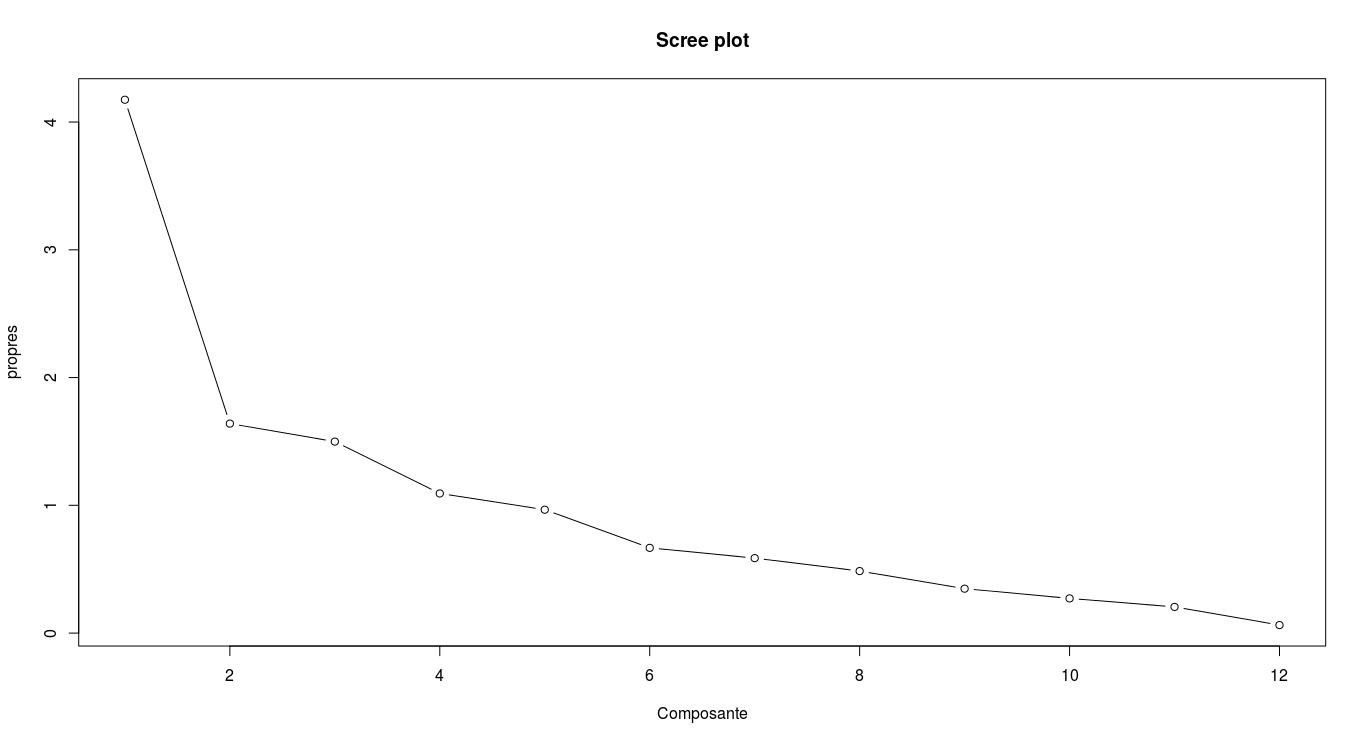
\includegraphics[width=\linewidth]{ch4-images/scree}}
						    		\caption{Graphe des éboulis de la décomposition spectrale de la matrice de corrélation}
						    		\label{fig:scree}
					\end{figure}
	La figure \ref{fig:inert} suivante montre que 70\% et 78\% de l'inertie de l'ensemble des données est expliquée par les 4 et 5 premières CP respectivement.
				\begin{figure}[H]
					    		\centering
					    		\fbox{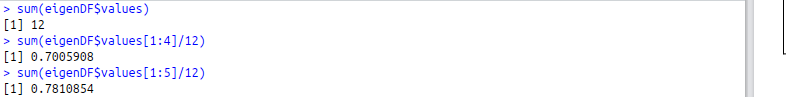
\includegraphics[width=\linewidth]{ch4-images/inertie}}
					    		\caption{Inertie expliquée par les 5 premières CP}
					    		\label{fig:inert}
				\end{figure}
	Puisque seulement les 4 premières CP possèdent des variances supérieures à une variable normée, i.e. il y'a 4 valeurs propres > 1. Nous procédons à la création des termes des combinaisons linéaires $Z_1,Z_2,Z_3,Z_4$ en utilisant les vecteurs propres correspondant.
	Les 4 facteurs ainsi créés, nous établissons leur corrélation à l'égard des variables intrantes de bases. La figure \ref{fig:ZZ} donne le résultat des corrélations variables-facteurs.
					\begin{figure}[H]
						    		\centering
						    		\fbox{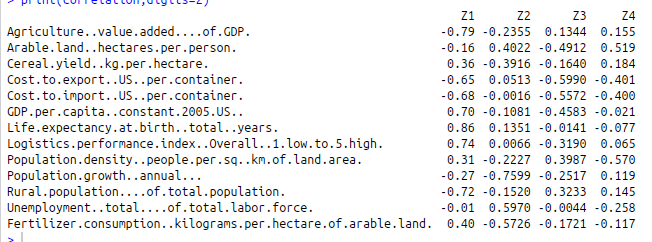
\includegraphics[width=\linewidth]{ch4-images/interpret}}
						    		\caption{Corrélations variables-facteurs}
						    		\label{fig:ZZ}
					\end{figure}	
	\begin{enumerate}
	\item Le facteur Z1 est:\begin{itemize}
		\item Négativement corrélé avec:\begin{itemize}
		\item La part de l'agriculture dans le PIB
		\item Les coûts d'import et exports
		\item La fraction rurale de la population
		\item La part de l'agriculture dans le PIB
		\end{itemize}
		\item Positivement corrélé avec:\begin{itemize}
		\item L'espèrance de vie
		\item L'indice de la performance logistique
		\item Le PIB par habitant
		\end{itemize}
		Z1 varie le plus entre les pays les plus riche, avec les meilleurs standards de la vie et les plus industrialisés d'une part, et d'une autre part les pays les plus pauvres, les plus dépendant de la culture agricole vivrière pour la nourriture et où les conditions de vie sont très durs. Comme le montre la carte des individus \ref{fig:inter3}, sur les valeurs positives, nous retrouvons les pays européens et sur les valeurs négatives, nous retrouvons les pays africains subsahariens pour la plupart. La consommation de fertilisants est positivement corrélées indiquant ainsi une tendances des pays riches, et non dépendants sur l'agriculture économiquement à utiliser plus d'engrais contrairement aux pays pauvre agricoles. Les fertilisants nécessitent des moyens financiers pour encourager la consommation. Le besoin environnemental ne suffit pas.
	\end{itemize}
	\item Le facteur Z2 est:\begin{itemize}
		\item Négativement corrélé avec:\begin{itemize}
		\item La croissance démographique annuelle.
		\item La consommation de fertilisants.
		\item Le rendement de la production céréalière.
		\end{itemize}
		\item Positivement corrélé avec:\begin{itemize}
		\item Le nombre d'hectares arables par personne
		\item Taux de chômage
		\end{itemize}
		Z2 varie le plus entre les pays les moins peuplés par rapport à la surface du pays et disposant d'assez de terres arables pour leur population en émigration à cause des perspectives professionnels non prometteuses d'une part, et d'autre part entre les pays où le moins de terres arables est diponible par habitant pour une économie en plein boom. Comme le montre la carte des individus \ref{fig:inter3}, sur les valeurs positives, nous retrouvons les pays de l'ex URSS et les Balkans, et sur les valeurs négatives, nous retrouvons les pays souffrant de peu de surfaces praticables pour l'agriculture disposés en archipels d’îles, des pays désertiques et qui connaissent une croissance démographique majeure. L'économie florissante de ces derniers avec des taux de chômage marginaux pour une population grandissante, favorise largement la consommation de fertilisants puisque ceux-ci se voient renforcés par deux facteurs qui s'imposent souvent : Les moyens financiers et la pression démographique sur les ressources naturelles.
		\end{itemize}
		Nous nous suffirons dans notre discussion uniquement du premier plan factoriel puisque Z3 et Z4 ne sont pas corrélés à notre variable endogène : \textbf{Consommation de kilogrammes de fertilisants phosphatés par hectare de terre arable} comme présenté sur la figure \ref{fig:ZZ}.
	\end{enumerate}
					\begin{figure}[H]
					\centering
					\fbox{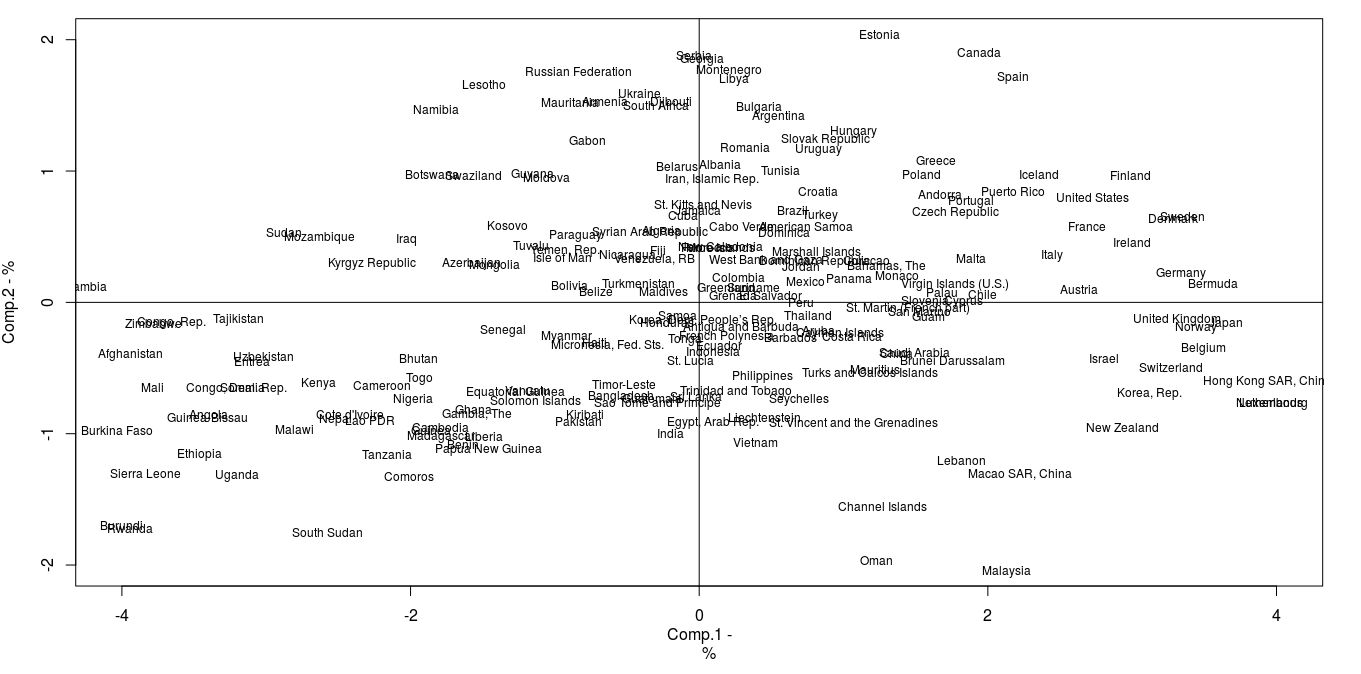
\includegraphics[width=1.1\linewidth]{ch4-images/interpret3}}
					\caption{Carte des individus}
					\label{fig:inter3}
					\end{figure}
			
	\section{Mise en œuvre: régression en composantes principales}
	Nous créons une nouvelle matrice des données composée de la variable endogène, \textbf{Consommation de kilogrammes de fertilisants phosphatés par hectare de terre arable} et des composantes principales.
	La figure \ref{fig:scatter2} ci-après présente la sortie de la matrice des corrélations croisée mais cette fois-ci entre la variable endogène et les CP.
				\begin{figure}[H]
					    		\centering
					    		\fbox{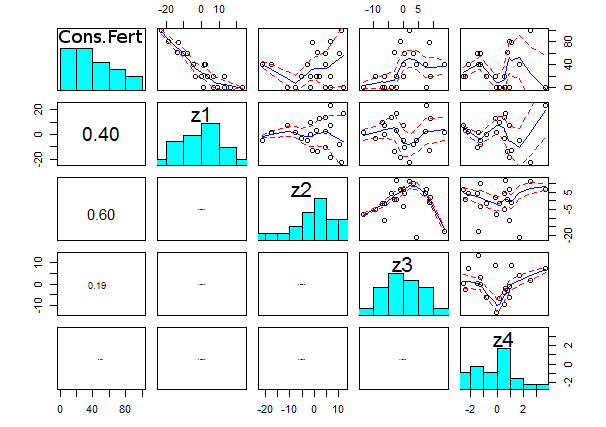
\includegraphics[width=.6\linewidth]{ch4-images/scatter2}}
					    		\caption{Diagrammes des dispersions croisées, courbes splines et corrélations des CPs}
					    		\label{fig:scatter2}
				\end{figure}
	Nous procédons par la suite à une régression linéaire multiple en utilisant les 4 CPs en tant que variables expliquatives de la \textbf{Consommation de kilogrammes de fertilisants phosphatés par hectare de terre arable}. La procédure et la sortie de cette régression est donnée par la figure \ref{fig:PCR} suivante :
					\begin{figure}[H]
						    		\centering
						    		\fbox{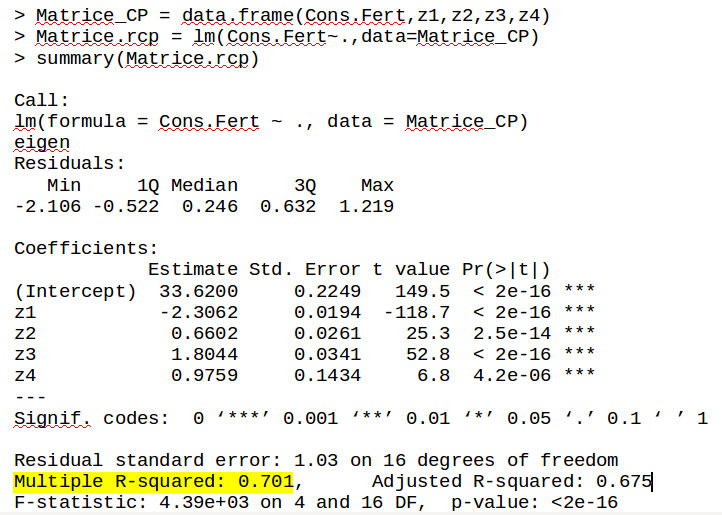
\includegraphics[width=.65\linewidth]{ch4-images/rcp}}
						    		\caption{Régression linéaire de Cons.Fert sur les CP}
						    		\label{fig:PCR}
					\end{figure}
	Les résidus que nous traçons sur la figure \ref{fig:residuals} se montrent remarquables compte tenu des relations non linéaires sur les graphes de la figure \ref{fig:scatter2}.
						\begin{figure}[H]
							    		\centering
							    		\fbox{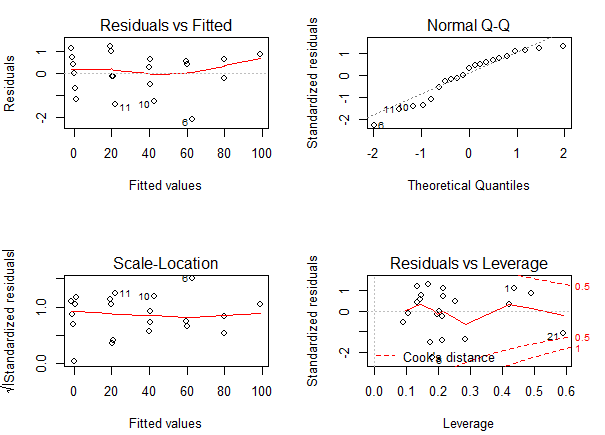
\includegraphics[width=.65\linewidth]{ch4-images/residuals}}
							    		\caption{Graphiques des résidus de la régression linéaire de Cons.Fert sur les CP}
							    		\label{fig:residuals}
						\end{figure}
	Nous avons retenu 7 échantillons des données originales que nous utilisons ici aux fins de validation et d'évaluation du modèle sur lequel nous réalisons un RMSE = 4.48.
							\begin{figure}[H]
								    		\centering
								    		\fbox{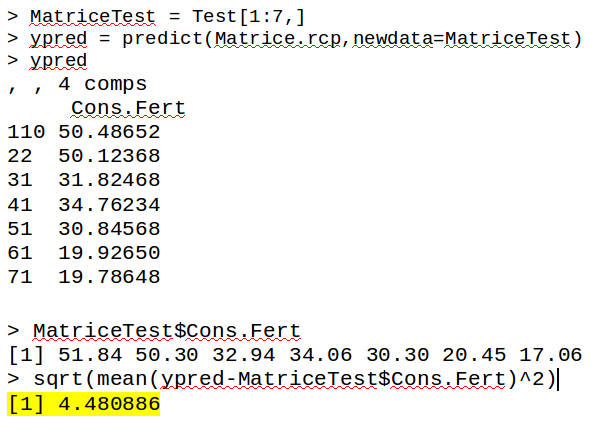
\includegraphics[width=.8\linewidth]{ch4-images/validation}}
								    		\caption{Validation du modèle et calcul du RMSE}
								    		\label{fig:residuals}
							\end{figure}
	